\documentclass[12pt]{report}
\usepackage[utf8]{inputenc}
\usepackage[T2A]{fontenc}
\usepackage[russian]{babel}
%\usepackage[14pt]{extsizes}
\usepackage{listings}
\usepackage{caption}
\usepackage{graphicx}
\usepackage{amsmath,amsfonts,amssymb,amsthm,mathtools}
\usepackage{pgfplots}
\usepackage{filecontents}
\usepackage{indentfirst}
\usepackage{eucal}
\usepackage{enumitem}
% Для \abs{}
\usepackage{commath}
\usepackage{float}
\frenchspacing


\usetikzlibrary{datavisualization}
\usetikzlibrary{datavisualization.formats.functions}

\usepackage[left=2cm,right=2cm, top=2cm,bottom=2cm,bindingoffset=0cm]{geometry}
% Для измененных титулов глав:
\usepackage{titlesec, blindtext, color} % подключаем нужные пакеты
\definecolor{gray75}{gray}{0.75} % определяем цвет
\newcommand{\hsp}{\hspace{20pt}} % длина линии в 20pt
% titleformat определяет стиль
\titleformat{\chapter}[hang]{\Huge\bfseries}{\thechapter\hsp\textcolor{gray75}{|}\hsp}{0pt}{\Huge\bfseries}

% plot
\usepackage{xcolor}
\usepackage{stmaryrd}
\usepackage{wasysym}
\usetikzlibrary{datavisualization}
\usetikzlibrary{datavisualization.formats.functions}

% листинги
\lstset{
    language=kotlin,
    basicstyle=\small\sffamily,
    numbers=left,
    numberstyle=\tiny,
    stepnumber=1,
    numbersep=5pt,
    showspaces=false,
    showstringspaces=false,
    showtabs=false,
    frame=single,
    tabsize=2,
    breaklines=true,
    breakatwhitespace=false,
    escapeinside={\#*}{*)},
}


\captionsetup[lstlisting]{singlelinecheck=false}



\begin{document}
%\def\chaptername{} % убирает "Глава"
    % Титульник
    \thispagestyle{empty}
    \begin{titlepage}
        \noindent \begin{minipage}{0.15\textwidth}
                      
\includegraphics[width=\linewidth]{img/b_logo}
        \end{minipage}
        \noindent\begin{minipage}{0.9\textwidth}
                     \centering
                     \textbf{Министерство науки и высшего образования Российской Федерации}\\
                     \textbf{Федеральное государственное бюджетное образовательное учреждение высшего образования}\\
                     \textbf{~~~«Московский государственный технический университет имени Н.Э.~Баумана}\\
                     \textbf{(национальный исследовательский университет)»}\\
                     \textbf{(МГТУ им. Н.Э.~Баумана)}
        \end{minipage}

        \noindent\rule{18cm}{3pt}
        \newline\newline
        \noindent ФАКУЛЬТЕТ $\underline{\text{«Информатика и системы управления»}}$ \newline\newline
        \noindent КАФЕДРА $\underline{\text{«Программное обеспечение ЭВМ и информационные технологии»}}$\newline\newline\newline\newline\newline


        \begin{center}
            \noindent\begin{minipage}{1.3\textwidth}
                         \centering
                         \Large\textbf{  Отчет по лабораторной работе №1}\newline
                         \textbf{по дисциплине "Анализ алгоритмов"}\newline\newline
            \end{minipage}
        \end{center}

        \noindent\textbf{Тема} $\underline{\text{Расстояние Левенштейна}}$\newline\newline
        \noindent\textbf{Студент} $\underline{\text{Тагилов А.М.}}$\newline\newline
        \noindent\textbf{Группа} $\underline{\text{ИУ7-55Б}}$\newline\newline
        \noindent\textbf{Оценка (баллы)} $\underline{\text{~~~~~~~~~~~~~~~~~~~~~~~~~~~}}$\newline\newline
        \noindent\textbf{Преподаватели} $\underline{\text{Волкова Л.Л., Строганов Ю.В.}}$\newline\newline\newline

        \begin{center}
            \vfill
            Москва~---~\the\year
            ~г.
        \end{center}
    \end{titlepage}

    \renewcommand{\contentsname}{Содержание}
    \tableofcontents

    % Введение
    \newpage
    \chapter*{Введение}
    \addcontentsline{toc}{chapter}{Введение}
    \textbf{Расстояние Левенштейна} --- минимальное количество операций вставки одного символа, удаления одного символа
    и замены одного символа на другой, необходимых для преобразования одной строки в другую.

    Расстояние Левенштейна применяется в теории информации и компьютерной лингвистике для:
    \begin{itemize}
        \item исправления ошибок в слове;
        \item сравнения текстовых файлов утилитой diff;
        \item сравнения генов, хромосом и белков в биоинформатике.
    \end{itemize}

    Задача поиска редакционного расстояния в современном мире является наиболее актуальной, так как зачастую необходимо
    предоставить пользователю возможность делать ошибки в интернет-запросах \cite{search}, указаниях инструкций к помощниками и т.д.
    Данный подход повышает уровень взаимодействия с пользователем и, соответственно, влияет на качество итогового
    программного продукта, а, чтобы алгоритм работал быстро и качественно, необходим правильный его выбор.
    Целью данной работы является изучить алгоритмы поиска редакционного расстояния и реализовать некоторые из возможных
    алгоритмов с использованием методов динамического программирования \cite{dp}.

    Для достижения поставленной цели необходимо выполнить следующие задачи:

    \begin{itemize}
        \item рассмотреть существующие алгоритмы поиска редакционного расстояния;
        \item провести сравнение и выявить достоинства и недостатки рассмотренных алгоритмов;
        \item привести схемы выбранных алгоритмов;
        \item определить средства для реализации алгоритмов;
        \item подготовить классы данных и ожидаемый результат для эксперимента и описать эксперимент;
        \item оценить алгоритмы по времени и памяти.
    \end{itemize}


    % Аналитическая часть
    \newpage


    \chapter{Аналитическая часть}

    Расстояние Левенштейна~\cite{levenshtein} между двумя строками ---
    минимальное количество операций вставки одного символа, удаления одного символа
    и замены одного символа на другой, необходимых для преобразования одной строки в другую.

    Цена каждой операции может зависеть от вида операции или от участвующих в ней символов, отражающих вероятность
    разных ошибок при вводе текста.
    \\
    Виды операций и их цены.
    \begin{enumerate}
        \item Вставка (insert), $w(a,\lambda)$ --- цена удаления символа $a$.
        \item Удаление (delete), $w(\lambda, b)$ --- цена вставки символа $b$.
        \item Замена (replace), $w(a, b)$ --- цена замены символа $a$ на символ $b$.
    \end{enumerate}

    Для решения задачи о нахождении редакционного расстояния необходимо найти последовательность операций, при которых
    суммарная цена операций будет минимальной. Расстояние Левенштейна - частный случай решения этой задачи
    при заданных условиях:
    \begin{itemize}
        \item $w(a, a) = 0$;
        \item $w(a, b) = 1, a \neq b$;
        \item $w(a, \lambda) = 1$;
        \item $w(\lambda, b) = 1$.
    \end{itemize}


    \section{Рекурсивный алгоритм нахождения расстояния Левенштейна}\label{sec:ReccursiveLev}
    В основе вычисления расстояние Левенштейна между двумя строками a и b лежит формула~\ref{eq:D},
    где:
    \begin{itemize}
        \item $\abs{a}$ означает длину строки $a$;
        \item $a[i]$ - \emph{i}-ый символ строки $a$.
    \end{itemize}

    \begin{equation}
        \label{eq:D}
        D(i, j) = \begin{cases}
                      0 &\text{i = 0, j = 0} \\
                      i &\text{j = 0, i > 0} \\
                      j &\text{i = 0, j >0} \\
                      \min \lbrace \\
                      \qquad D(i, j - 1) + 1 \\
                      \qquad D(i - 1, j) + 1 &\text{i > 0, j > 0} \\
                      \qquad D(i - 1, j - 1) + m(a[i], b[j]) &\text{\ref{eq:m}} \\
                      \rbrace
        \end{cases}
    \end{equation}

    Функция 1.2 позволяет сравнить два символа:
    \begin{equation}
        \label{eq:m}
        m(a, b) = \begin{cases}
                      0 &\text{a = b} \\
                      1 &\text{иначе}
        \end{cases}
    \end{equation}

    Рекурсивный алгоритм реализует формулу~\ref{eq:D}.
    Логика функции $D$ состоит в следующем.
    \begin{enumerate}
        \item Для получения из пустой строки пустой строки, требуется 0 операций.
        \item Для получения из пустой строки строки $b$ требуется \abs{b} операций (все - insert).
        \item Для получения из строки $a$ пустой строки требуется \abs{a} операций (все - delete).
        \item Для получения из строки $a$ строки $b$ требуется выполнить несколько операций.
        Обозначая $a'$ и $b'$ за строки $a$ и $b$ без последнего символа соответсвенно, цену преобразования
        из строки $a$ в $b$ можно выразить следующим образом.
        \begin{enumerate}
            \item Сумма цены преобразования строки $a'$ в $b$ и цены операции удаления (для преобразования $a'$ в $a$).
            \item Сумма цены преобразования строки $a$ в $b'$ и цены операции вставки (для преобразования $b'$ в $b$).
            \item Сумма цены преобразования строки $a'$ в $b'$ и операции замены
            (если a и b оканчиваются на разные символы).
            \item Цена преобразования строки $a'$ в $b'$ (если $a$ и $b$ оканчиваются на одинаковый символ).
        \end{enumerate}
        Минимальная цена преобразования --- минимальное значение из приведенных выше вариантов.
    \end{enumerate}


    \section{Итерационный алгоритм нахождения расстояния Левенштейна с использованием матрицы}
    Прямая реализация формулы~\ref{eq:D} может быть неэффективна при больших значениях длин строк,
    поскольку промежуточные значения функции $D(i, j)$ вычисляются несколько раз.
    Для оптимизации алгоритма можно использовать матрицу для хранения промежуточных значений функции $D(i, j)$.
    В таком случае алгоритм выполняет построчное заполнение матрицы, пока не дойдет до крайнего правого элемента,
    в котором будет записано итоговое расстояние Левенштейна.


    \section{Рекурсивный алгоритм нахождения расстояния Левенштейна с использованием матрицы}
    Основной недостаток обычного рекурсивного алгоритма --- многократное вычисления промежуточных значений
    функции D(i, j).
    Этот недостаток можно устранить, и сделать таким образом алгоритм более эффективным по времени выполнения,
    если добавить матрицу, которая будет заполняться промежуточными значениями D(i, j).
    Если рекурсивный алгоритм обрабатывает данные, которые еще ни разу не были поданы, результат
    записывается в матрицу.
    Если рекурсивный алгоритм обрабатывает данные, которые уже были обработаны, берется старый результат из матрицы.


    \section{Расстояние Дамерау-Левенштейна}
    Расстояние Дамерау-Левенштейна очень похоже на расстояние Левенштейна, но в его поиске используется еще одна
    операция - \textbf{транспозиция} (перестановка двух соседних символов).

    Расстояние Дамерау-Левенштейна между двумя строками a и b определяется функцией~\ref{eq:dl}:

    \begin{equation}
        \label{eq:dl}
        d_{a, b}(i, j) =
        \begin{cases}
            \max(i, j)
            & \text{если } \min(i, j) = 0
            \\
            \min
            \begin{cases}
                d_{a, b}(i - 1, j) + 1
                \\
                d_{a, b}(i, j - 1) + 1
                \\
                d_{a, b}(i - 1, j - 1) + m(a[i], b[j])
                \\
                d_{a, b}(i - 2, j - 2) + 1
            \end{cases}
            & \begin{aligned}
                  \text{если } i, j > 1 \\ \text{и } a[i] = b[j - 1] \\ \text{ и } a[i - 1] = b[j]
            \end{aligned}
            \\
            \min
            \begin{cases}
                d_{a, b}(i - 1, j) + 1
                \\
                d_{a, b}(i, j - 1) + 1
                \\
                d_{a, b}(i - 1, j - 1) + m(a[i], b[j])
            \end{cases}
            & \text{иначе}
            \\
        \end{cases}
    \end{equation}
    Формула выводится по тем же соображениям, что и~\ref{eq:D}. Прямое применение рекурсивной функции тоже
    неэффективно по времени исполнения, так что аналогично методу, описанному в~\ref{sec:ReccursiveLev}
    добавляется матрица для хранения промежуточных значений.


    \section{Вывод}
    В данном разделе были рассмотрены алгоритмы нахождения расстояния Левенштейна и Дамерау-Левенштейна.
    Формулы Левенштейна и Дамерау-Левенштейна для нахождения расстояния между строками задаются рекурсивно
    и программно могут быть реализованы как рекурсивно, так и итерационно.

    \newpage


    \chapter{Конструкторская часть}

    В данном разделе выбранные алгоритмы будут формализованы в виде блок-схем.

    \section{Схемы алгоритмов}
    В данной части будут рассмотрены схемы алгоритмов нахождения расстояния Левенштейна и Дамерау-Левенштейна.
    На рисунках \ref{fig:levRecur} - \ref{fig:levDamCasual} представлены рассматриваемые алгоритмы.

    \begin{figure}[H]
        \centering
        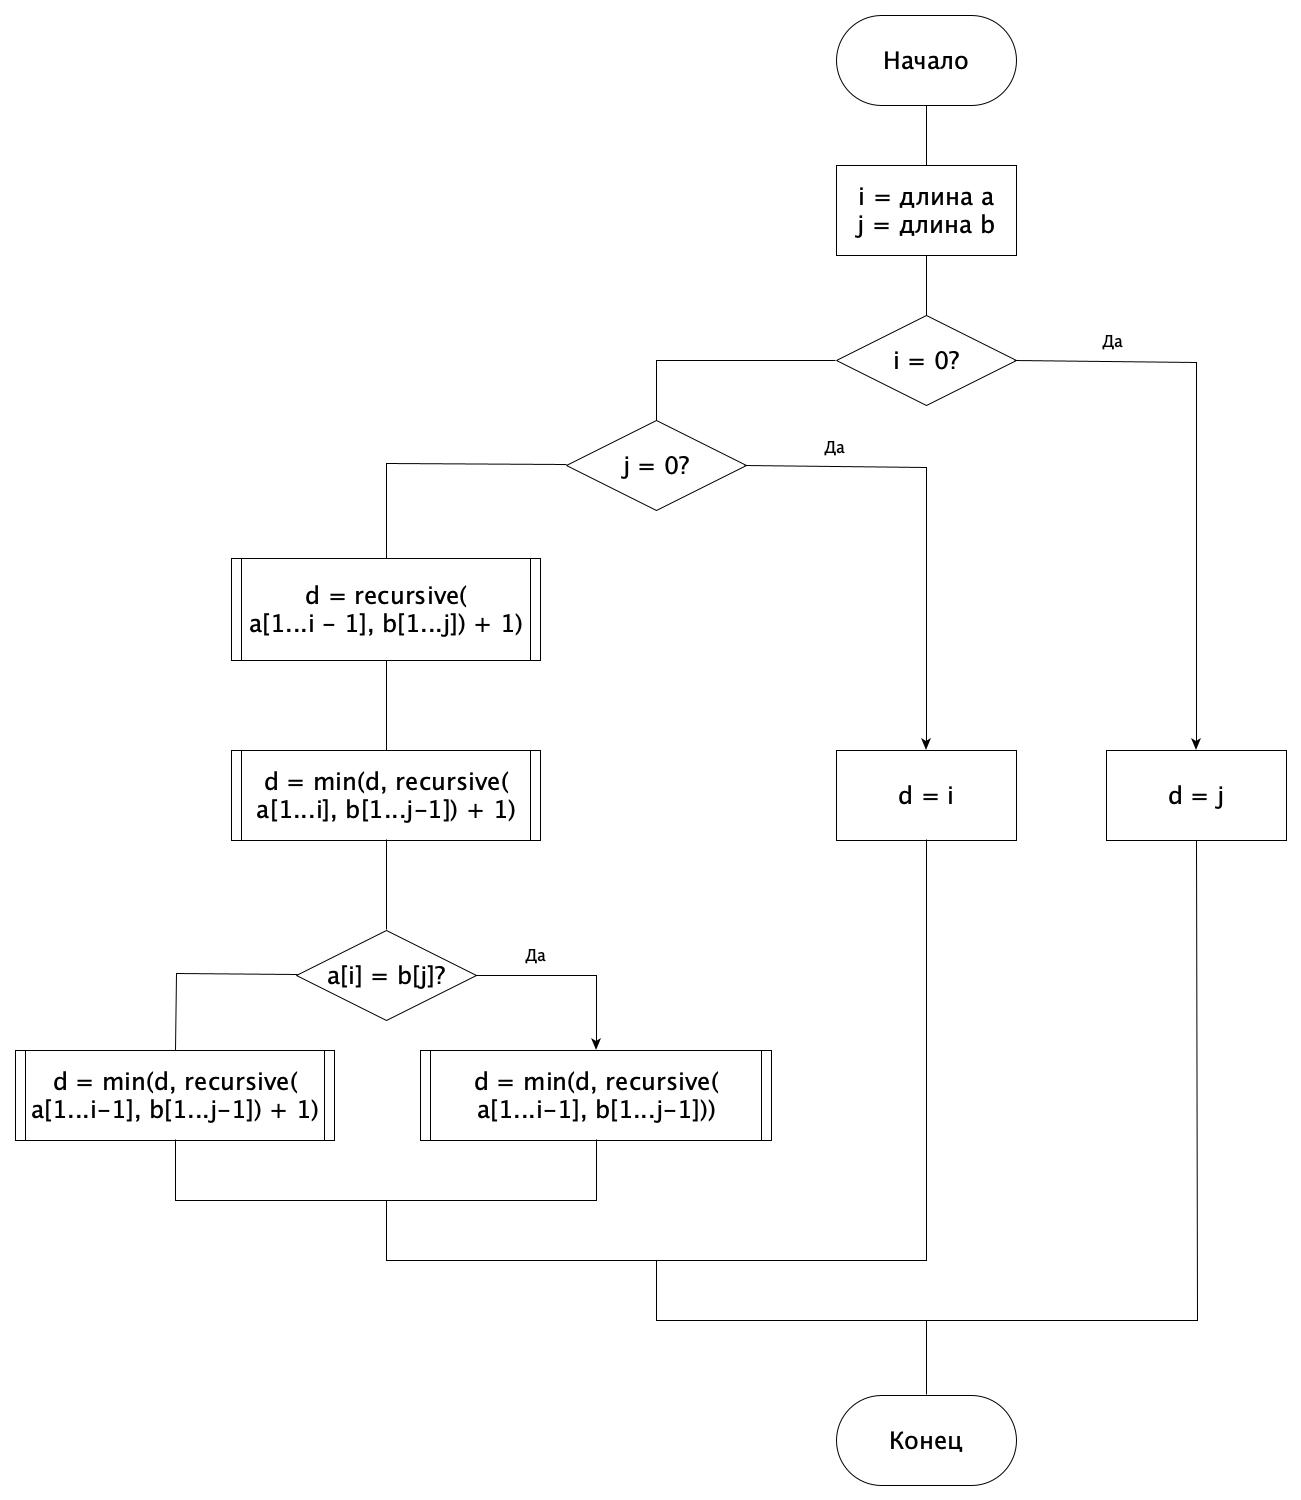
\includegraphics[width=0.7\linewidth]{img/levRecur}
        \caption{Блок-схема рекурсивного агоритма нахождения расстояния Левенштейна}
        \label{fig:levRecur}
    \end{figure}

    \begin{figure}[H]
        \centering
        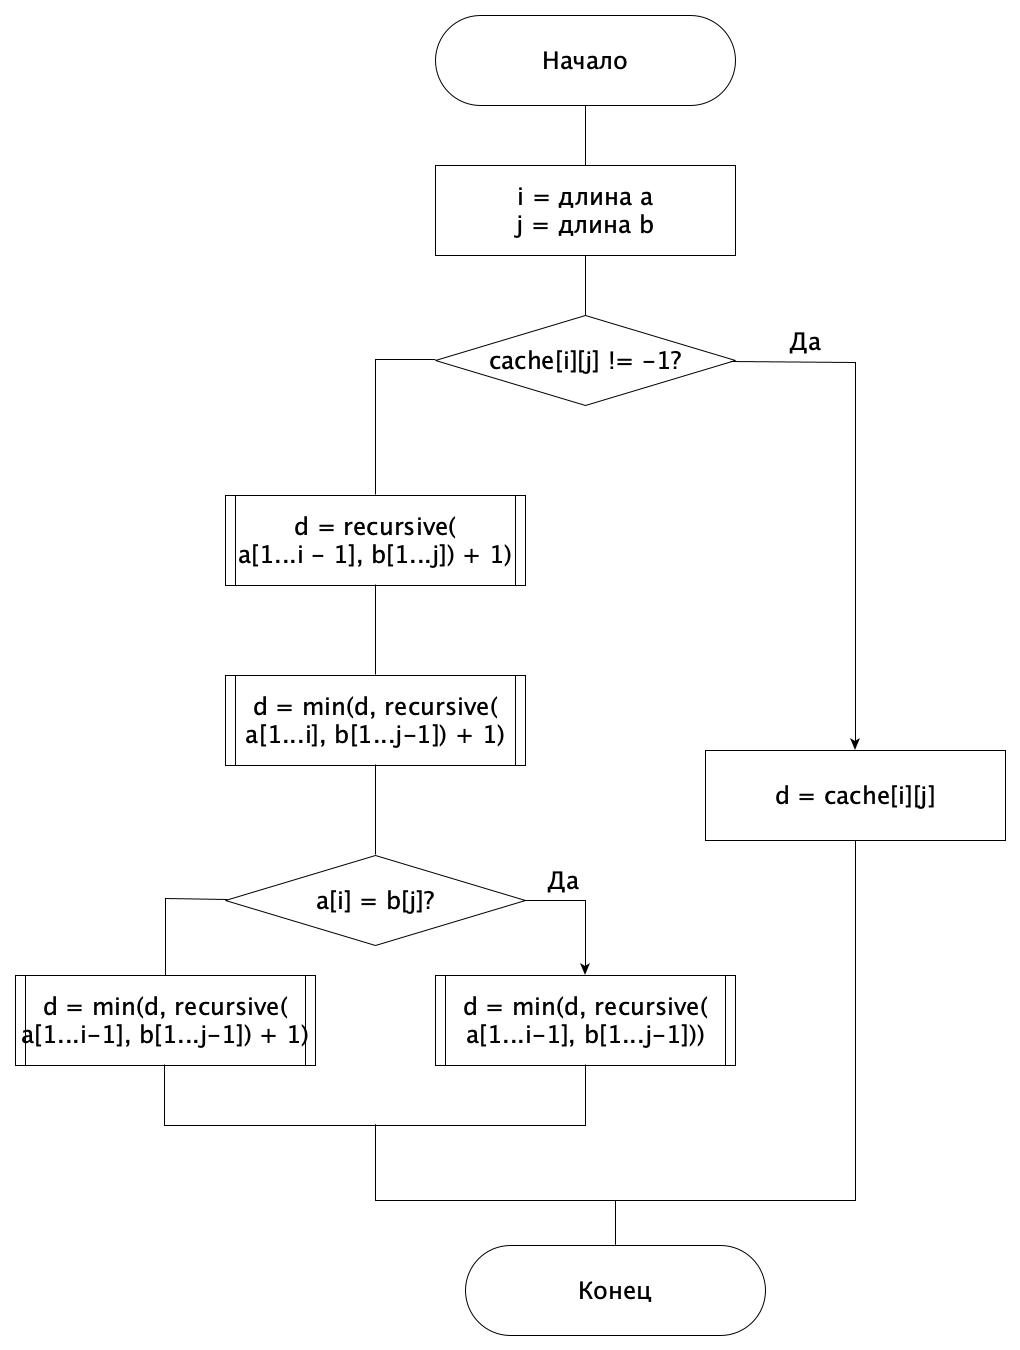
\includegraphics[width=0.7\linewidth]{img/levRecurCache}
        \caption{Блок-схема рекурсивного агоритма нахождения расстояния Левенштейна с использованием матрицы}
        \label{fig:levRecurCache}
    \end{figure}


    \begin{figure}[H]
        \centering
        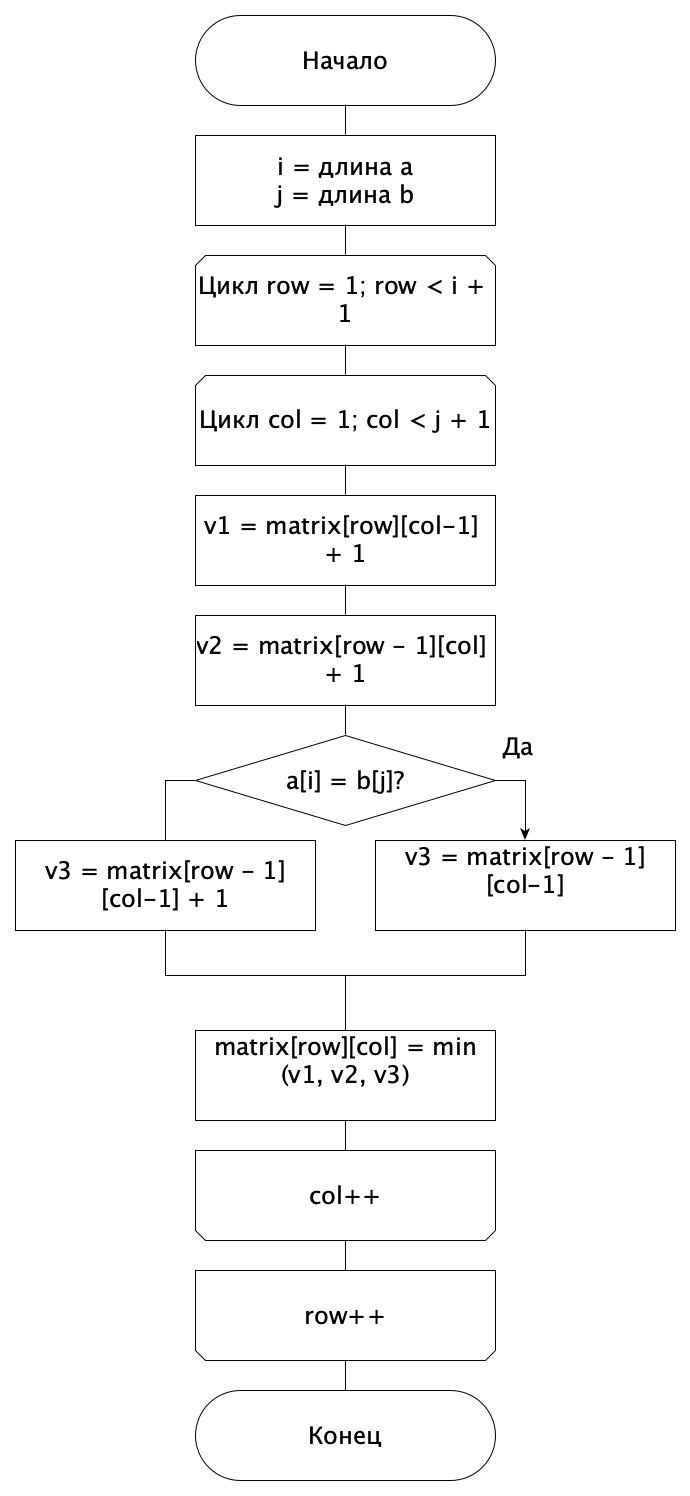
\includegraphics[width=0.6\linewidth]{img/levCasual}
        \caption{Блок-схема итерационного агоритма нахождения расстояния Левенштейна}
        \label{fig:levCasual}
    \end{figure}


    \begin{figure}[H]
        \centering
        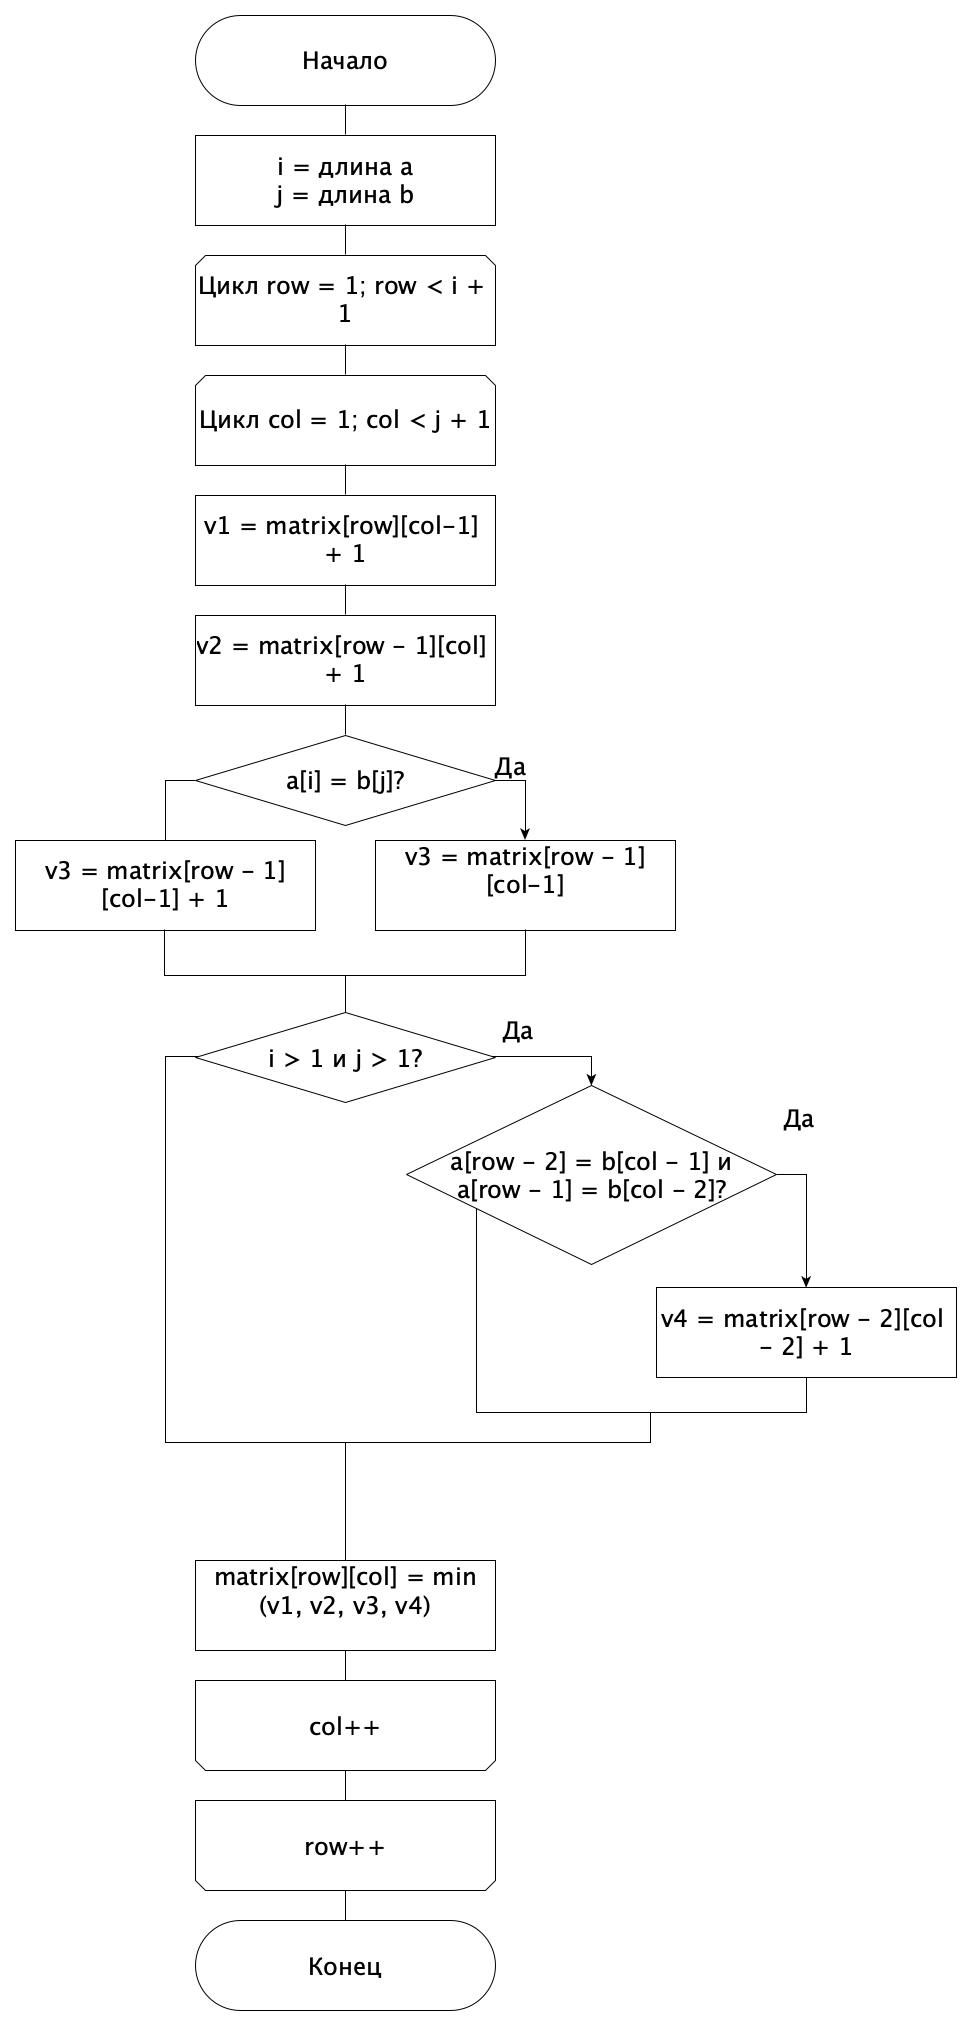
\includegraphics[width=0.6\linewidth]{img/levDamCasual}
        \caption{Блок-схема итерационного агоритма нахождения расстояния Дамерау-Левенштейна}
        \label{fig:levDamCasual}
    \end{figure}


    \section{Вывод}
    На основе теоретических данных, полученных в аналитическом разделе,
    были построены блок-схемы исследуемых алгоритмов


    \chapter{Технологическая часть}


    \section{Требования к ПО}
    К разрабатываемому программному обеспечению предъявляются следующие требования:
    \begin{enumerate}
        \item Подготовить тесты поиска расстояния между строками.
        \item ПО должно выводить количество использованного процессорного времени.
        \item ПО должно работать корректно.
    \end{enumerate}


    \section{Средства реализации}
    Для реализации программы нахождения расстояния Левенштейна и Дамерау-Левенштейна
    я выбрал язык программирования Kotlin~\cite{kotlin}. Такой выбор обусловлен широкими возможностями языка.
    Несмотря на то, что данный язык программирования только набирает популярность, его не коснулась проблема
    недостатка библиотек, как как он работает поверх Java Virtual Machine - можно использовать библиотеки из Java.



    \section{Реализация алгоритмов}
    В листингах приведена реализация алгоритмов нахождения расстояния Левенштейна и Дамерау-Левенштейна.
    \begin{lstlisting}[label={lst:algbase},caption=Базовый класс для всех алгоритмов]
abstract class Algorithm() {
    open val name: String = "Abstract algorithm"
    protected var s1: String = ""
    protected var s2: String = ""
    public open val isDam: Boolean = false
    public abstract fun findDiff(): Int
    public fun setData(str1: String, str2: String) {
        s1 = str1
        s2 = str2
    }
}
    \end{lstlisting}

    \begin{lstlisting}[label={lst:levrecur},caption=Метод для нахождения расстояния Левенштейна рекурсивно,
        language=kotlin]
class LevRecursionAlgorithm(): Algorithm() {
    override val name = "Levenshtein Recursive"
    override fun findDiff(): Int {
        return findDiff(s1.length, s2.length)
    }
    private fun findDiff(l1: Int, l2: Int): Int {
        if (l1 == 0) return l2
        if (l2 == 0) return l1
        val match: Int = if (s1[l1 - 1] == s2[l2 - 1]) 0 else 1
        val insertion: Int = findDiff(l1 - 1, l2) + 1
        val deletion: Int = findDiff(l1, l2 - 1) + 1
        val substitution: Int = findDiff(l1 - 1, l2 - 1) + match
        return minOf(insertion, deletion, substitution)
    }
}
    \end{lstlisting}

    \begin{lstlisting}[label={lst:levrecurmatrix},caption=Метод для нахождения расстояния Левенштейна рекурсивно
    \(\text{с матрицей}\),language=kotlin]
class LevMatrixAlgorithm(): Algorithm() {
    override val isDam = false
    override val name = "Levenshtein Recursive with cache"

    var array: Array<Array<Int>>? = null
    override fun findDiff(): Int {
        array = Array(s1.length + 1) { Array(s2.length + 1) { -1 } }
        return findDiff(s1.length, s2.length)
    }
    private fun findDiff(l1: Int, l2: Int): Int {
        if (array!![l1][l2] != -1)
            return array!![l1][l2]
        if (l1 == 0) return l2
        if (l2 == 0) return l1
        val match: Int = if (s1[l1 - 1] == s2[l2 - 1]) 0 else 1
        val insertion: Int = findDiff(l1 - 1, l2) + 1
        val deletion: Int = findDiff(l1, l2 - 1) + 1
        val substitution: Int = findDiff(l1 - 1, l2 - 1) + match
        val result = minOf(insertion, deletion, substitution)
        array!![l1][l2] = result
        return result
    }
}
    \end{lstlisting}

    \begin{lstlisting}[label={lst:levсasualmatrix},caption=Метод для нахождения расстояния Левенштейна итерационно,
        language=kotlin]
class LevIterAlgorithm(): Algorithm() {
    override val name = "Levenshtein Iterable"
    override val isDam = false
    override fun findDiff(): Int {
        val array = Array(2) { Array(s2.length + 1) { -1 } }
        array[0].forEachIndexed { index, _ -> array[0][index] = index }
        for (index in 1..s1.length) {
            val i = 1
            if (index > 1) {
                array[0] = array[1]
                array[1] = Array(s2.length + 1) { -1 }
            }
            array[1][0] = index
            for (j in 1..s2.length) {
                val valueUp = array[i - 1][j] + 1
                val valueLeft = array[i][j - 1] + 1
                val diagMatch = if (s1[index - 1] == s2[j - 1]) 0 else 1
                val valueDiag = array[i - 1][j - 1] + diagMatch
                array[i][j] = minOf(valueUp, valueLeft, valueDiag)
            }
        }
        return array[1][s2.length]
    }
}
    \end{lstlisting}

    \begin{lstlisting}[label=code:levDamRecursion,caption=Метод для нахождения расстояния Дамерау-Левенштейна
    рекурсивно,language=kotlin]
class DamRecursionAlgorithm(): Algorithm() {
    override val name = "Damerau-Levenshtein Recursive"
    override fun findDiff(): Int {
        return findDiff(s1.length, s2.length)
    }
    private fun findDiff(l1: Int, l2: Int): Int {
        if (l1 == 0) return l2
        if (l2 == 0) return l1
        val match: Int = if (s1[l1 - 1] == s2[l2 - 1]) 0 else 1
        val insertion: Int = findDiff(l1 - 1, l2) + 1
        val deletion: Int = findDiff(l1, l2 - 1) + 1
        var substitution: Int = findDiff(l1 - 1, l2 - 1) + match
        var result: Int = minOf(insertion, deletion, substitution)
        if (l1 > 1 && l2 > 1 && s1[l1 - 1] == s2[l2 - 2] && s1[l1 - 2] == s2[l2 - 1])
            result = minOf(findDiff(l1 - 2, l2 - 2) + 1, result)
        return result
    }
}
    \end{lstlisting}

    \begin{lstlisting}[label=code:levDamRecursionCache,caption=Метод для нахождения расстояния Дамерау-Левенштейна
    рекурсивно \(\text{с матрицей}\),language=kotlin]
class DamMatrixAlgorithm(): Algorithm() {
    var array: Array<Array<Int>>? = null
    override val name = "Damerau-Levenshtein Recursive with cache"
    override fun findDiff(): Int {
        array = Array(s1.length + 1) { Array(s2.length + 1) { -1 } }
        return findDiff(s1.length, s2.length)
    }
    private fun findDiff(l1: Int, l2: Int): Int {
        if (array!![l1][l2] != -1)
            return array!![l1][l2]
        if (l1 == 0) return l2
        if (l2 == 0) return l1
        val match: Int = if (s1[l1 - 1] == s2[l2 - 1]) 0 else 1
        val insertion: Int = findDiff(l1 - 1, l2) + 1
        val deletion: Int = findDiff(l1, l2 - 1) + 1
        val substitutionOrSwap: Int = findDiff(l1 - 1, l2 - 1) + match
        var result = minOf(insertion, deletion, substitutionOrSwap)
        if (l1 > 1 && l2 > 1 && s1[l1 - 1] == s2[l2 - 2] && s1[l1 - 2] == s2[l2 - 1])
            result = minOf(findDiff(l1 - 2, l2 - 2) + 1, substitutionOrSwap, result)
        array!![l1][l2] = result
        return result
    }
}
    \end{lstlisting}

    \begin{lstlisting}[label=code:levDamCasual,caption=Метод для нахождения расстояния Дамерау-Левенштейна
    итерационно,language=kotlin]

class DamIterAlgorithm(): Algorithm() {
    override val name = "Damerau-Levenshtein Iterable"
    override fun findDiff(): Int {
        val array = Array(3) { Array(s2.length + 1) { -1 } }
        array[0].forEachIndexed { index, _ -> array[0][index] = index }
        for (index in 1..s1.length) {
            var i = index
            if (index > 2) {
                array[0] = array[1]
                array[1] = array[2]
                array[2] = Array(s2.length + 1) { -1 }
                i = 2
            }
            array[1][0] = index - 1
            array[2][0] = index
            for (j in 1..s2.length) {
                val valueUp = array[i - 1][j] + 1
                val valueLeft = array[i][j - 1] + 1
                val diagMatch = if (s1[index - 1] == s2[j - 1]) 0 else 1
                val valueDiag = array[i - 1][j - 1] + diagMatch
                var result = minOf(valueUp, valueLeft, valueDiag)
                if (index > 1 && j > 1 && s1[index - 2] == s2[j - 1] && s1[index - 1] == s2[j - 2])
                    result = minOf(result, array[0][j - 2] + 1)
                array[i][j] = result
            }
        }
        if (s1.length > 2)
            return array[2][s2.length]
        else
            return array[s1.length][s2.length]
    }
}
    \end{lstlisting}


    \section{Тестовые данные}
    В таблице~\ref{tab:tests} приведены тестовые данные, на которых было протестировано разработанное ПО.

    \begin{table}[H]
        \centering
        \caption{Тестовые данные}
        \label{tab:tests}
        \begin{tabular}{|c c c c c|}
            \hline
            № & Первое слово & Второе слово & Ожидаемый результат & Полученный результат \\ [0.8ex]
            \hline
            1 & кит          & кот         & 1, 1                & 1, 1                 \\
            \hline
            2 & собака       & собачка     & 4, 2                & 4, 2                 \\
            \hline
            3 & dija         & djia         & 4, 4                & 4, 4                 \\
            \hline
            4 &              &              & 0, 0                & 0,0                  \\
            \hline
            5 &              & абв          & 3, 3                & 3, 3                 \\
            \hline
            6 & абв          &              & 3, 3                & 3, 3                 \\
            \hline
            7 & увлечение        & развлечения        & 4, 4                & 4, 4                 \\
            \hline
        \end{tabular}
    \end{table}


    \section{Вывод}
    В данном разделе были разработаны исходные коды шести алгоритмов: вычисления расстояния
    Левенштейна и Дамерау-Левенштейна рекурсивно, рекурсивно с матрицей и итерационно


    \chapter{Исследовательская часть}



    \section{Пример работы программы}
    Демонстрация работы программы приведена на рисунке \ref{fig:workSample}

    \begin{figure}[H]
        \centering
        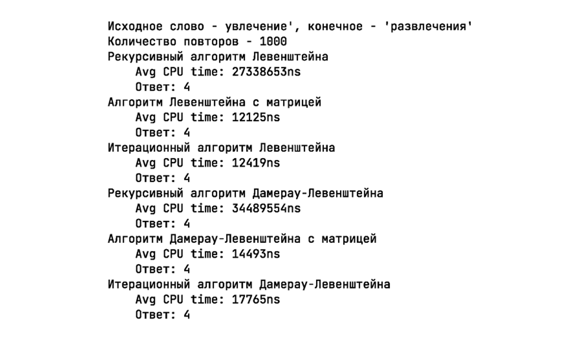
\includegraphics[scale=1]{img/workSample}
        \caption{Демонстрация работы программы}
        \label{fig:workSample}
    \end{figure}


    \section{Технические характеристики}
    Ниже приведены технические характеристики устройства, на котором было проведено тестирование ПО:
    \begin{itemize}
        \item операционная система --- Mac OS Big Sur 11.4;
        \item процессор --- Intel(R) Core(TM) i5-7267U CPU @ 2.90GHz \cite{i5};
        \item оперативная память --- 8 GB.
    \end{itemize}


    \section{Оценка времени алгоритмов}
    Kotlin работает поверх Java Virtual Machine, поэтому возможно использование Java библиотек~\cite{kotlin}.
    Время выполнения алгоритмов замерялось с помощью Java-интерфейса для управления потоками
    виртуальной машины Java - ThreadMXBean~\cite{threadMXBean}, позволяющего вычислить процессорное время,
    затраченное на определенный процесс.

    В таблице~\ref{tab:times} представлены замеры времени работы для каждого из алгоритмов. Для всех алгоритмов
    время было усреднено по результатам 1000 замеров. Слова являлись случайным набором символов.

    \begin{table}[H]
        \caption{Таблица времени выполнения алгоритмов (в наносекундах)}
        \label{tab:times}
        \centering
        \begin{tabular}{|c c c c c c c|}
            \hline
            Длина строк & LevRec & LevRecMatrix   & LevIter & LevDamRec & LevDamRecMatrix & LevDamIter  \\
            \hline
            10          & 27432321     & 13730 & 20106        & 36903970       & 24900 & 27488           \\
            \hline
            20          & ---    & 33711      & 45668        & ---      & 85596       & 69764          \\
            \hline
            50          & ---   & 85698      & 94424        & ---      & 137873       & 163268         \\
            \hline
            100         & ---   & 317519      & 213333      & ---     & 407036       & 248863         \\
            \hline
        \end{tabular}
    \end{table}

    \begin{figure}[H]
        \centering
        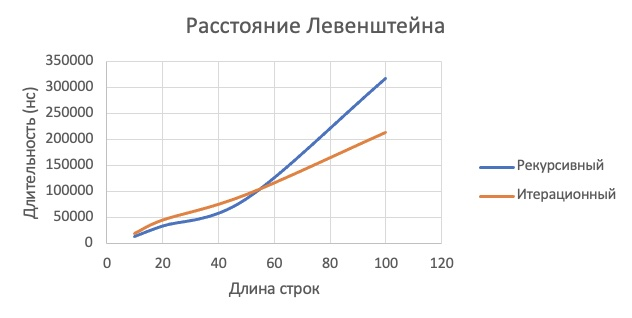
\includegraphics[scale=0.75]{img/levGraphic}
        \caption{График времени выполнения алгоритмов поиска расстояния Левенштейна}
        \label{fig:levGraphic}
    \end{figure}

    \begin{figure}[H]
        \centering
        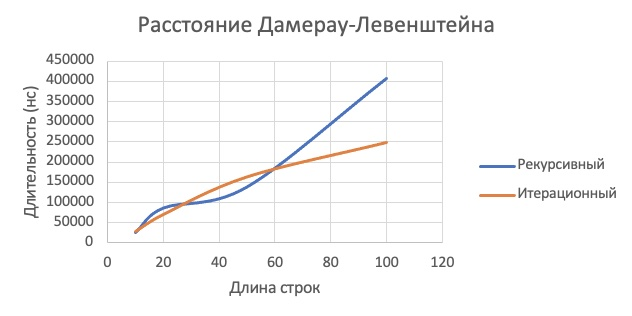
\includegraphics[scale=0.75]{img/levDamGraphic}
        \caption{График времени выполнения алгоритмов поиска расстояния Дамерау-Левенштейна}
        \label{fig:levDamGraphic}
    \end{figure}

    \section{Использование памяти}
    Алгоритмы нахождения расстояний Левенштейна и Дамерау-Левенштейна практически
    не отличаются друг от друга с точки зрения используемой памяти.

    Максимальная глубина стека вызовов при рекурсивной реализации --- сумма длин входных строк.
    Тогда максимальный объем требуемой памяти равен:

    \begin{equation}
        (len(Str_{1}) + len(Str_{2})) \cdot
        (2 \cdot K(String) + 7 \cdot K(int)),
    \end{equation}
    $len$ --- оператор вычисления длины строки,
    $Str_{1}$ и $Str_{2}$ --- входные строки,
    где $K$ --- оператор вычисления размера,
    $String$ --- строковый тип, $int$ --- целочисленный тип.

    Объем используемой памяти при итерационной реализации равен (при оптимизации матрицы до 2 строк):
    \begin{equation}
        2 \cdot (len(Str_{2}) + 1) \cdot K(int) +
        4 \cdot K(int)
    \end{equation}


    \section{Вывод}
    Рекурсивные реализации алгоритмов нахождения расстояний Левенштейна и Дамерау-Левенштейна
    работают дольше итерационных реализаций при длине слов от 60 символов: при длине в 100 символов итерационные
    алгоритмы справляются почти в два раза быстрее. Для меньшей длины разумно использовать рекурсивные алгоритмы.
    Время работы реализаций увеличивается в геометрической прогрессии.
    Рекурсивный алгоритм с матрицей работает немногим медленнее итерационного: для 100 символов разница составила
    порядка 30\% для расстояния Левенштейна и порядка 40 \% для Дамерау-Левенштейна.
    \chapter*{Заключение}
    \addcontentsline{toc}{chapter}{Заключение}
    В ходе проделанной работы был изучен метод динамического программирования на материале реализации
    алгоритмов нахождения расстояний Левенштейна и Дамерау-Левенштейна.
    Были изучены алгоритмы поиска расстояний Левенштейна и Дамерау-Левенштейна и получены навыки
    реализации указанных алгоритмов в матричной и рекурсивных версиях, в том числе и с кэшированием результатов.

    Экспериментально подтверждено различие во временной эффективности рекурсивной и итерационной
    реализаций алгоритмов поиска расстояний Левенштейна и Дамерау-Левенштейна
    при помощи разработанного программного обеспечения с замерами процессорного времени.
    Рекурсивные реализации оказались быстрее при длине слов до 60 символов, в остальных случаях
    итерационные показали уменьшение длительности работы до двух раз при длине слов в 100 символов.

    Теоретически было рассчитано использование памяти в каждой из реализаций алгоритмов поиска
    расстояний Левенштейна и Дамерау-Левенштейна. Рекурсивный алгоритм с матрицей (кэшированием)
    использует больше всего памяти.

    \newpage
    \addcontentsline{toc}{chapter}{Список литературы}

    \bibliographystyle{utf8gost705u}  % стилевой файл для оформления по ГОСТу
    \bibliography{report_1}          % имя библиографической базы (bib-файла)

\end{document}